\documentclass[tikz]{standalone}
\usepackage{tikz}
\usetikzlibrary{positioning, graphs}
\usetikzlibrary{graphs.standard}
\usetikzlibrary{arrows.meta}
\begin{document}
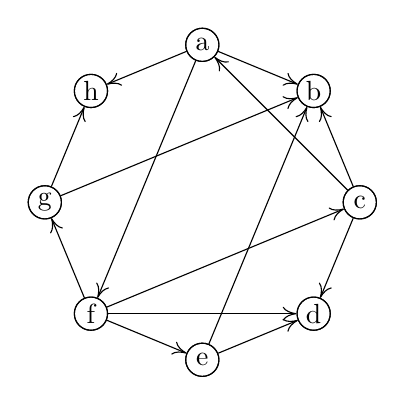
\begin{tikzpicture}
\begin{scope}
		[every node/.style={draw,circle,inner sep = 0em, minimum size = 1.2em},
		 edgelabel/.style = {fill = white, inner sep = 0.1em, font=\small}]
		\graph[clockwise, radius = 2cm, phase = 0, empty nodes]{subgraph I_n[n = 8, name = A]};
		
		\node at (A 7) {a};
		\node at (A 8) {b};
		\node at (A 1) {c};
		\node at (A 2) {d};
		\node at (A 3) {e};
		\node at (A 4) {f};
		\node at (A 5) {g};
		\node at (A 6) {h};
		
		\draw[-{>[length=5, width=5]}] (A 1) to (A 7);
		\draw[-{>[length=5, width=5]}] (A 1) to (A 2);
		\draw[-{>[length=5, width=5]}] (A 1) to (A 8);
		\draw[-{>[length=5, width=5]}] (A 3) to (A 2);
		\draw[-{>[length=5, width=5]}] (A 3) to (A 8);
		\draw[-{>[length=5, width=5]}] (A 4) to (A 1);
		\draw[-{>[length=5, width=5]}] (A 4) to (A 2);
		\draw[-{>[length=5, width=5]}] (A 4) to (A 3);
		\draw[-{>[length=5, width=5]}] (A 4) to (A 5);
		\draw[-{>[length=5, width=5]}] (A 5) to (A 6);
		\draw[-{>[length=5, width=5]}] (A 5) to (A 8);
		\draw[-{>[length=5, width=5]}] (A 7) to (A 8);
		\draw[-{>[length=5, width=5]}] (A 7) to (A 4);
		\draw[-{>[length=5, width=5]}] (A 7) to (A 6);
\end{scope}
\end{tikzpicture}
\end{document}